% !Author = JustinMa
% !Date = 5/19/25

\documentclass[12pt]{article}

% Packages
\usepackage{amsmath}
\usepackage{graphicx}
\usepackage{booktabs}
\usepackage{caption}
\usepackage{float}
\usepackage{tikz}
\usepackage{setspace}
\usepackage{times}
\usepackage[left=1in, right=1in, top=1in, bottom=1in]{geometry}

\doublespacing

% TikZ libraries and styles
\usetikzlibrary{shapes.geometric, arrows.meta, positioning, shadows}

\tikzset{
    layer/.style={
        rectangle,
        draw=black!80,
        rounded corners,
        minimum width=5cm,
        minimum height=0.6cm,
        text centered,
        text width=7cm,
        font=\small,
        drop shadow,
        fill=#1
    },
    arrow/.style={
        -{Stealth[length=2mm]},
        thick,
        shorten >=2pt,
        shorten <=2pt
    }
}

\begin{document}

    \centerline{\textbf{Investigating Overfitting in Convolutional Neural Networks}}

    \noindent\textbf{1. Introduction}

    Neural networks are a form of machine learning models, roughly inspired by how the human brain
    processes information. They have become increasingly prevalent in our developing world, providing
    powerful and unique solutions to a wide variety of problems. However, with power also comes risk,
    as training a neural network too much on a small dataset can cause overfitting. Overfitting occurs
    when a model learns the training data too well by essentially memorizing it, causing it to perform
    well on data in its training set but poorly on unseen data. While it might seem that simply
    increasing a model’s size would always boost accuracy by allowing it to capture more patterns,
    extra parameters often give the network enough capacity to store the training set outright, allowing
    it to overfit. Smaller networks, by contrast, are forced to find the underlying patterns in the data
    because of their limited size. In this study, we investigate whether increasing the number of parameters
    in a convolutional neural network leads to greater overfitting when trained on a small dataset, as
    measured by the difference between training and test accuracy.

    \noindent\textbf{2. Statistical Question}

    Does increasing the number of parameters in a fixed CNN architecture cause a greater difference
    between training and testing accuracy?

    \noindent\textbf{Hypotheses:}\newline
    \centerline{$H_0: \beta = 0$} \newline
    \centerline{$H_a: \beta > 0$} \newline
    Where $\beta$ is the true slope of the population least‐squares regression line that relates number
    of parameters of the model to the difference in accuracy of the model on the train dataset and the
    test dataset.

    \noindent\textbf{3. Data Collection}

    We trained $\mathbf{x}$ convolutional models on a randomly selected small subset of size 100 images
    from the CIFAR-10 dataset, each with the same architecture (\textit{see figure 1}). Each model had
    a different number of parameters, roughly uniformly ranging from approximately 1 million to 50 million.
    We controlled the parameter count by multiplying the amount of filters for the Conv2D layers and the amount of units
    for the hidden Dense layers by a scalar factor, $n$.
    For each model, the initial values of the parameters are randomly set, so each model can be seen as randomly
    selected from all possible models of that size and architecture before training.

    \noindent\textbf{Model Architecture}
    \begin{center}
        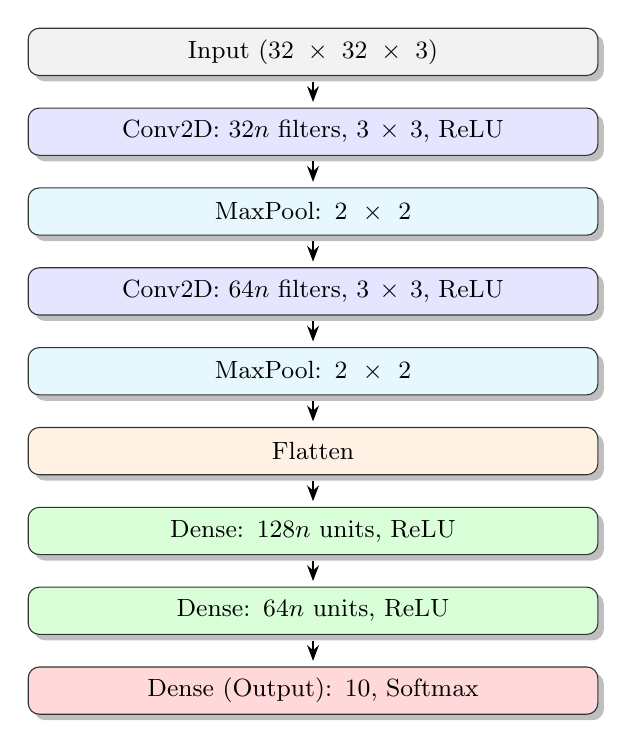
\begin{tikzpicture}[node distance=4mm and 0mm]
            \node[layer=gray!10]                     (input)  {Input $(32\times32\times3)$};
            \node[layer=blue!10,  below=of input]    (conv1)  {Conv2D: $32n$ filters, $3\times3$, ReLU};
            \node[layer=cyan!10,  below=of conv1]    (pool1)  {MaxPool: $2\times2$};
            \node[layer=blue!10,  below=of pool1]    (conv2)  {Conv2D: $64n$ filters, $3\times3$, ReLU};
            \node[layer=cyan!10,  below=of conv2]    (pool2)  {MaxPool: $2\times2$};
            \node[layer=orange!10,below=of pool2]    (flat)   {Flatten};
            \node[layer=green!15, below=of flat]    (dense1) {Dense: $128n$ units, ReLU};
            \node[layer=green!15, below=of dense1]  (dense2) {Dense: $64n$ units, ReLU};
            \node[layer=red!15,   below=of dense2]  (output) {Dense (Output): 10, Softmax};

            \draw[arrow] (input)  -- (conv1);
            \draw[arrow] (conv1)  -- (pool1);
            \draw[arrow] (pool1)  -- (conv2);
            \draw[arrow] (conv2)  -- (pool2);
            \draw[arrow] (pool2)  -- (flat);
            \draw[arrow] (flat)   -- (dense1);
            \draw[arrow] (dense1) -- (dense2);
            \draw[arrow] (dense2) -- (output);
        \end{tikzpicture}
    \end{center}

    \centerline{\textit{Figure 1: General Architecture of Our Models}}

    \noindent\textbf{Data Display}

    \noindent\textbf{Data Analysis}

    \noindent\textbf{Conclusion}

    \noindent\textbf{Reflection}

\end{document}
